\begin{titlepage}
    \begin{center}

        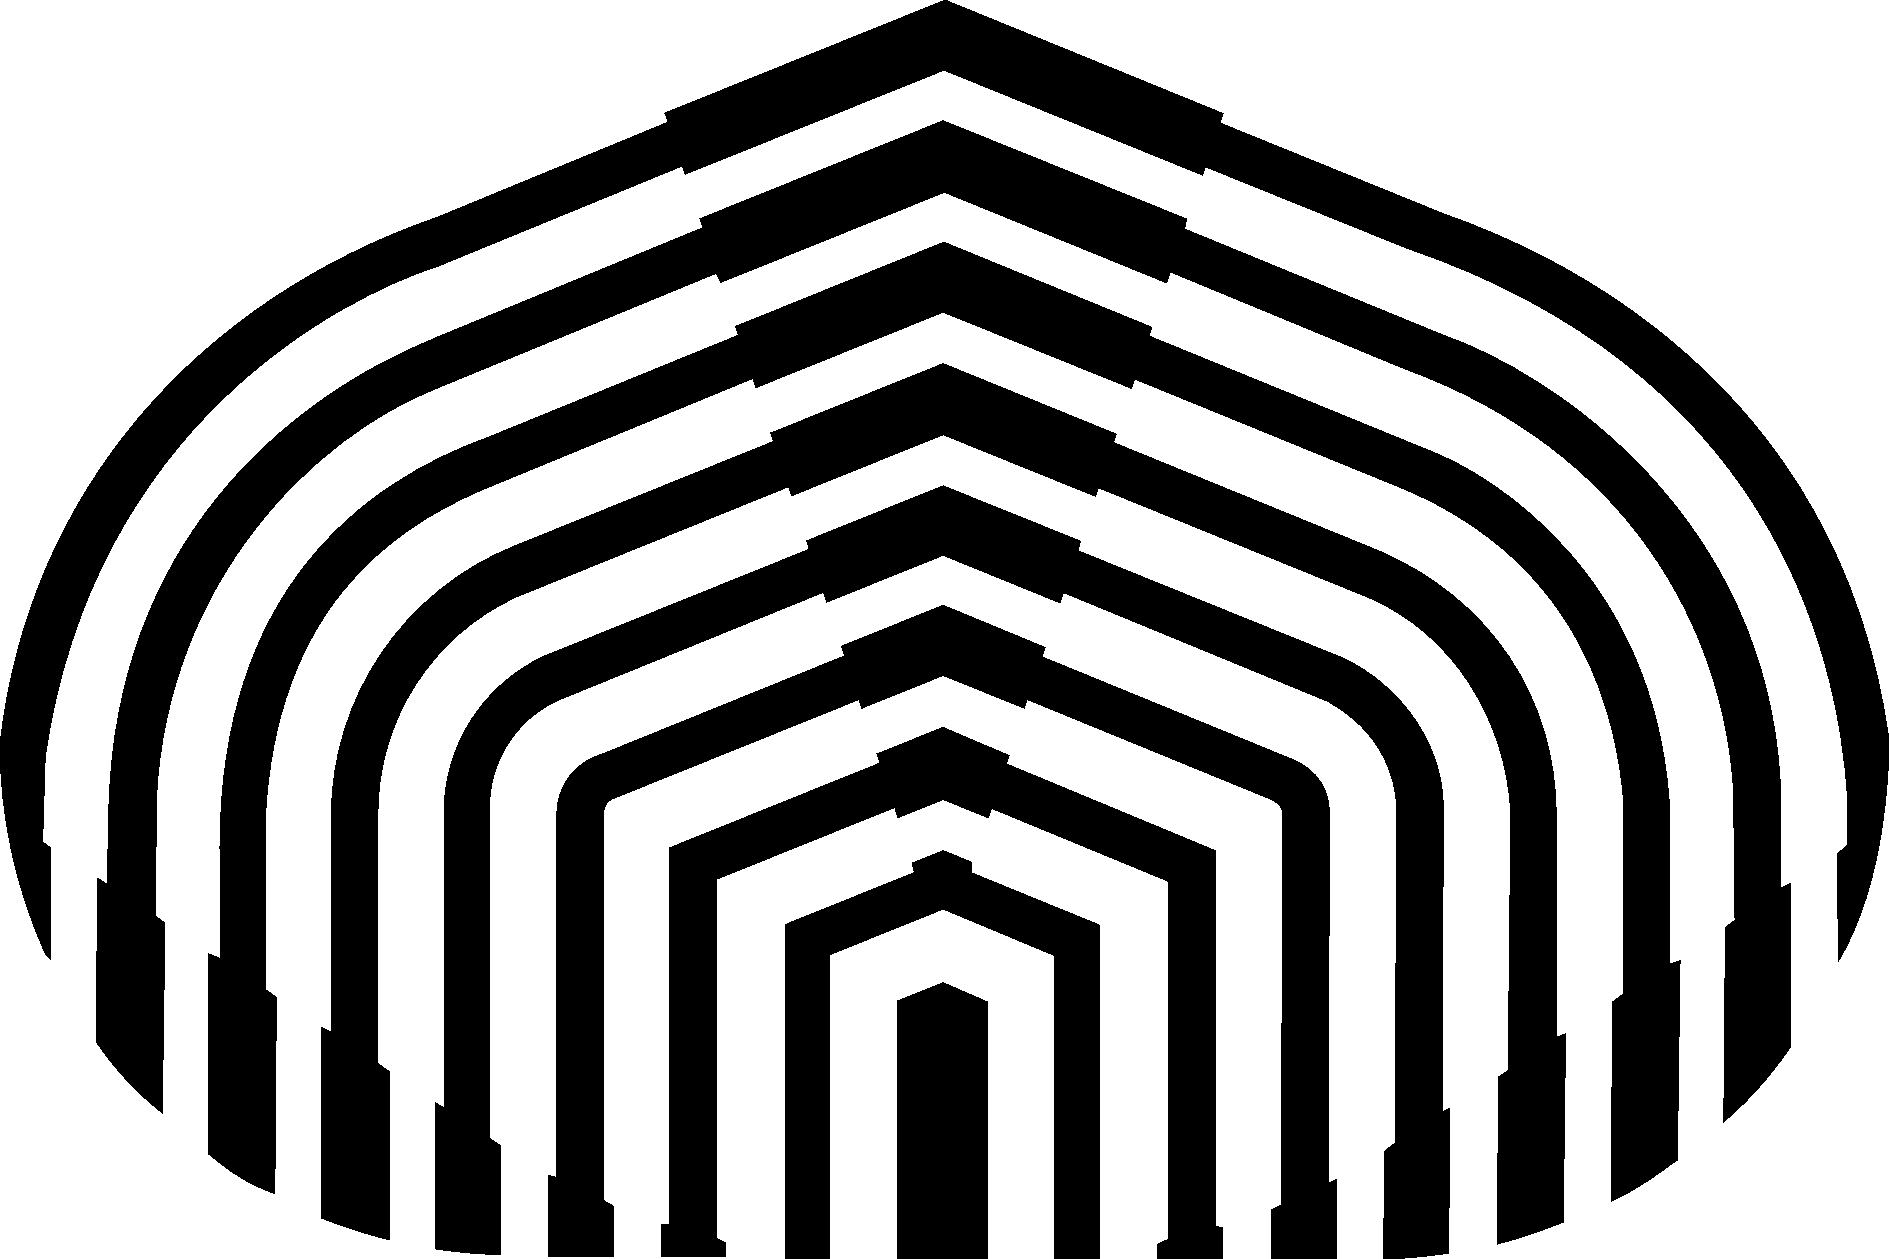
\includegraphics[scale=0.5]{usb.png} \\
        \textsc {\large UNIVERSIDAD SIMÓN BOLÍVAR} \\
        \textsc{DECANATO DE ESTUDIOS PROFESIONALES\\
        COORDINACIÓN DE INGENIERÍA ELECTRÓNICA}\\
        \textbf{SISTEMA DE GENERACIÓN DE MOSAICOS 2D PARA ROBOTS MÓVILES A PARTIR DE VIDEO MONOCULAR} \\
        PROYECTO DE GRADO \\
        PRESENTADO POR: \\
        Victor Yovanni Garcia Carmona, Carnet: 12-10738

    \end{center}
% El resumen debe ser de una sola página
\addtotoc{Resumen}
\abstract
{
    \addtocontents{toc}{\vspace{1em}}
    Al realizar tareas de exploración para el análisis de espacios aereos o de fondo marino, es muy comun emplear sistemas de adquisición basados en captura de videos para su posterior análisis. En la actualidad, el incremento de la tecnologia sobre el procesamiento de datos, ha permitido que los algoritmos de vision por computadora coloquen a la camara como principal sensor para la reconstruccion de entornos recorridos por vehiculos móviles. El presente trabajo tiene como finalidad el analisis y la implementación de distintos algoritmos para la reconstrucción de un mosaico 2D (dos dimensiones), a partir de la información proveniente de una camara monocular ubicada en la parte inferior de un robot. En la primera sección se describen las tecnicas utilizadas en la actualidad para la elaboración de mapas del suelo, con un gran enfoque en aplicaciones desafiantes como lo es, el mapeo de suelo subacuático. Posteriormente se detallará la implementación de distintos algoritmos usando tecnicas de procesamiento de imagenes y vision por computadora que permiten mejorar la detección de puntos clave, con el fin de optimizar el calculo de las matrices de transformación para la alineación de imagenes en un mosaico. Finalmente se muestran resultados, producto de un sistema automatizado, además del analisis de estos sistemas sobre el error de reproyección de imagenes en un mapa del suelo.
    
}

% Las palabras clave son generalmente los nombres de áreas de investigación a
% los cuales está asociado el trabajo. Generalmente son tres o cuatro.
\noindent \begin{small} \textbf{Palabras clave}: mosaico, video monocular, puntos clave, matriz de transformación. 
\end{small}
	
% Iniciar nueva página luego del resumen
\clearpage
\setstretch{1.3}

\end{titlepage}